
\section{The Mandelbrot set using OpenMP \punkte{25}}

Two executables were produced for this task.  The serial code \texttt{mandel\_seq.c} walks every pixel of the complex plane in raster order, iterating $z \leftarrow z^2 + c$ until the magnitude exceeds 2 or \texttt{MAX\_ITERS} is reached.  Every pixel stores its iteration count in a scratch buffer and the global counter \texttt{nTotalIterationsCount} is updated so that the statistics suggested in the assignment (iterations/second and MFlop/s) can be reported.  The parallel code \texttt{mandel\_par.c} keeps the same numerical kernel but wraps the pixel loop inside \verb|#pragma omp parallel for| with private temporaries and a \verb|reduction(+ : nTotalIterationsCount)|.  The image is written only after the parallel region to avoid races on the PNG writer.  The helper script \texttt{run\_mandel.sh} recompiles both binaries for four resolutions ($1024^2$, $2048^2$, $4096^2$, $8192^2$), runs the serial version once per size, and then launches the OpenMP version with \texttt{OMP\_NUM\_THREADS} $\in$ \{1,2,4,8,16,20\}.  Each run stores a log in \texttt{Skeleton\_codes/mandel/logs/} and the corresponding PNG in \texttt{Skeleton\_codes/mandel/png/}.

\begin{figure}[H]
    \centering
    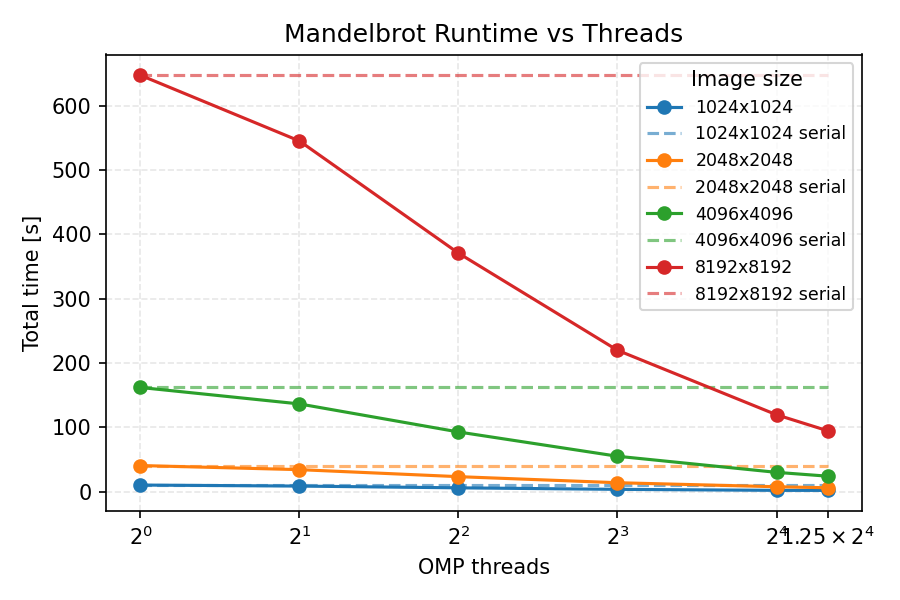
\includegraphics[width=0.75\linewidth]{../Skeleton_codes/mandel/plots/mandel_runtime_scaling.png}
    \caption{Total runtime versus thread count.}
    \label{fig:mandel_scaling}
\end{figure}

Example outputs for the two largest resolutions are shown in Figure~\ref{fig:mandel_images}.
\begin{figure}[H]
    \centering
    \begin{subfigure}{0.45\linewidth}
        
\includegraphics[width=\linewidth]{../Skeleton_codes/mandel/png/mandel_4096x4096_T20.png}
        \caption{4096×4096, 20 threads}
    \end{subfigure}
    \hfill
    \begin{subfigure}{0.45\linewidth}
        \includegraphics[width=\linewidth]{../Skeleton_codes/mandel/png/mandel_8192x8192_T20.png}
        \caption{8192×8192, 20 threads}
    \end{subfigure}
    \caption{Mandelbrot renderings generated by the OpenMP version.}
    \label{fig:mandel_images}
\end{figure}

Table~\ref{tab:mandel_times} summarises the measured times (seconds) for the OpenMP binary; the serial baseline corresponds to the entry with one thread.
\begin{table}[H]
    \centering
    \begin{tabular}{c|rrrrrr}
        \hline
        Image size & Sequential & 2 threads & 4 threads & 8 threads & 16 threads & 20 threads \\
        \hline
        1024×1024 & 10.13 & 8.54 & 5.80 & 3.44 & 1.88 & 1.80 \\
        2048×2048 & 40.48 & 34.09 & 23.18 & 13.74 & 7.49 & 5.91 \\
        4096×4096 & 161.92 & 136.35 & 92.72 & 54.93 & 29.89 & 23.93 \\
        8192×8192 & 647.71 & 545.44 & 370.92 & 219.81 & 119.51 & 94.57 \\
        \hline
    \end{tabular}
    \caption{Total runtime for the OpenMP version; the iteration count remains constant across threads for each resolution.}
    \label{tab:mandel_times}
\end{table}

The curves in Figure~\ref{fig:mandel_scaling} show that we achieve a speedup of roughly 5.6× on 20 threads for the smallest image and about 6.8× for the larger resolutions.  The dashed baselines overlap with the measured points at one thread, confirming that the OpenMP implementation does not introduce extra overhead beyond the parallel region.  Scaling flattens earlier for small images because there is less work per pixel and threads compete for memory bandwidth; at 8192² the per-thread workload is larger and the speedup remains close to linear.  In every case the iteration counter and the number of pixels reported in the logs match the expectations, which validates both the numerical kernel and the performance statistics requested in the assignment.
